\chapter{Hardware}

Now that we have covered the necessary mathematical background of the main algorithm used in this thesis, we will move on to an overview of the rover's design. 
%TODO: Mention initial parts list was inspired by http://www.instructables.com/id/Autonomous-Lynxmotion-Rover/
\section{Specific Hardware Used} \label{sectionSpecificHardware}
The hardware used in this project was chosen to minimize cost while producing a vehicle capable of navigating rough outdoors terrain. Parts that were already on hand, and that most college students would reasonably have access to, such as a personal laptop and an Android smartphone, were used over superior alternatives. In total these parts were purchased for less than \$500, with most of that cost coming from the rover's base rather than its sensors.

\begin{wrapfigure}{R}{0.25\textwidth} %this figure will be at the right
	\caption{\cite{fig_lynxmotion_rover}}
	\centering
	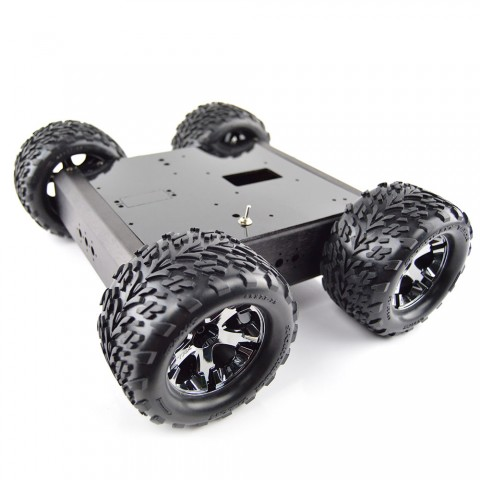
\includegraphics[width=0.25\textwidth]{lynxmotion-aluminum-a4wd1-rover-kit-w-encoders-7}
	\label{FigLynxmotionRover}
\end{wrapfigure}

The mobile base chosen was the Lynxmotion A4WD1 Rover, shown in Figure \ref{FigLynxmotionRover}. It was purchased as a kit including four 200 RPM DC gear motors, four 100 PPR motor encoders, and four 4.75" diameter wheels. The motor encoders are sensors which measure the rotation of the motors, and thus of the wheels. The chassis consists of four aluminum side brackets, and polycarbonate top and bottom panels. This kit made up the bulk of the rover's cost. It was chosen for its large wheels and strong motors, increasing the rover's robustness to uneven terrain and ramps. The chassis can support up to 5 lbs overall, and a second stackable level is available as an extension. While not purchased, this second level would be an ideal place to put a tablet or small laptop.

One downside of this base is the fixed position of the four wheels. The lack of a turnable axis means the rover must steer by varying the speed of its motors. This causes wheel slippage in one or more of the wheels when the rover turns, meaning the motor encoders do not see the distance traveled. This ultimately causes greater error buildup in the robot's localization. Choosing a different base which only uses two wheels would avoid this issue, and likely be cheaper. However, such a choice must be balanced with the robot's suitability for outdoor use, and room for all on-board components.

% also mention how this driver steps up the voltage from the arduino - that's why we need it
The motors are controlled by a Sabertooth 12A 6V-24V regenerative motor driver. There is a 5A version of this motor driver, which should have been purchased to save \$20. This driver is dual-channeled, i.e. it controls two separate motor channels. Two DC motors are attached to each channel, so that the left and right side wheels of the rover are each controlled by a single channel. The Sabertooth drives DC motors from these channels in a relatively simple way. The speed of DC motors is proportional to the voltage supplied to them, and the direction of rotation can be flipped simply by flipping the polarity of the supplied voltage. So the motor driver manages speed by modifying the voltage supplied to each channel. To do so it uses a technique called pulse-width modulation, which involves switching the power on and off at a high frequency. This approximates a smooth waveform of the average voltage and current. To change the direction of rotation, an on-board circuit called the H-bridge is used to flip the polarity of voltage supplied. \cite{dcMotorBlog}

%the motor driver protects from back EMF causing a current flow

The motor driver is powered by two LG 18650 HE2 rechargable lithium ion cells, which sit in a battery case. This case was made out of an 18650 battery holder soldered in series to act as a pack. The battery cells were individually charged before each use by a NiteCore-i2-V2014 li-ion charger. The Sabertooth motor driver has built-in lithium ion over-discharge protection, which ensures that the cells will not be discharged beyond their maximum capacity.

\begin{wrapfigure}{L}{0.25\textwidth} %this figure will be at the right
	\caption{\cite{fig_ping}}
	\centering
	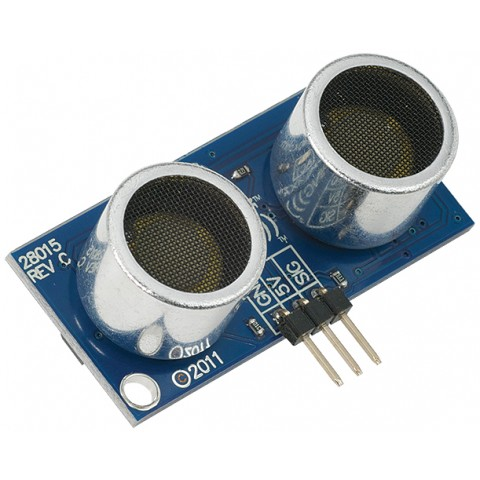
\includegraphics[width=0.25\textwidth]{parallax-ping-ultrasonic-sensor}
	\label{FigPing}
\end{wrapfigure}

Situated on top of the rover is the PING))) ultrasonic distance sensor (see Figure \ref{FigPing}), which is attached to a Parallax servo which pans back and forth 180 degrees. This range sensor emits an ultrasonic chirp, and times how long it takes for that chirp to echo back. Based on that time, the distance from the sensor to an obstacle can be calculated. The PING))) sensor can be used to detect objects from 2cm to 3 meters away. \cite{pingDocumentation}

\begin{wrapfigure}{R}{0.25\textwidth}
	\caption{\cite{fig_arduino_uno}}
	\centering
	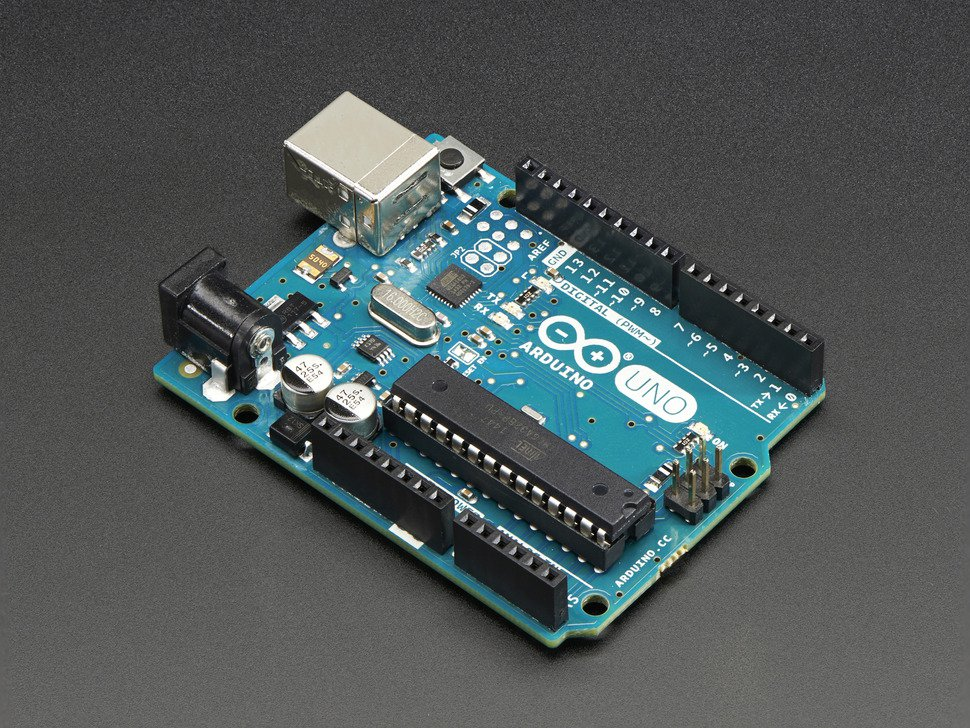
\includegraphics[width=0.25\textwidth]{arduinoUno}
	\label{FigArduino}
\end{wrapfigure}

At the heart of the rover is an Arduino Uno R3, shown in Figure \ref{FigArduino}. This microcontroller board handles low level control of the rover. It is hooked up to every other electronic on the rover by its input and output pins. It commands the motor driver, telling it at what speed to set the two output channels, and directly controls the panning motion of the Parallax servo. It also transmits sensor measurements to the computer. It is connected to this computer via a USB cable, which powers the board and allows communication over a serial port. Motor encoder values and ultrasonic range data are transmitted, and motor speed commands are received. An Arduino prototyping shield was stacked on top for soldering connections, to allow re-usability of the board.

Only two of the four available motor encoders are used, due to a limit of the microcontroller board used. Choosing a different model with more hardware interrupt pins would improve localization accuracy, without drastically increasing the price.

The computer used is a Dell Inspiron 3531 laptop, which has a quad-core 2.16 GHz processor, and 4 GB of RAM. Any personal laptop running Ubuntu or Debian could be used here, and additional computational resources would be beneficial. However, this laptop was a personal work machine and already available to use at no additional cost. The laptop is used as the main processing unit.

The last component in the design is a Nexus 4 smartphone placed on top of the rover, behind the ultrasonic sensor. Just like the Arduino board, it is connected to the laptop by USB. Inside this phone is an MPU-6050 chip which contains a digital gyroscope and accelerometer. Elsewhere on the phone's logic board is a magnetometer, otherwise known as a digital compass, and a GPS receiver. This was also a personal device already available, which acts as a cheap Inertial Measurement Unit (IMU) and GPS receiver for the robot.

Both USB cables used are just under 10 feet long. The USB 2.0 specification limits the length of cable between two 2.0 USB devices to less than five meters, or about 16 feet \cite{usbForum}. Thus there should be no connectivity problems given the current length, but the cables cannot be extended much further. 

Connecting electronics on the rover to the laptop via USB means the processing laptop must be manually kept within 10 feet of the rover as it navigates. Thus the rover is not truly autonomous. It could be made so by including wireless or radio communication with a server, or by using a larger chassis which would be able to simply carry the laptop. However, USB cables are cheap, and the current design still functions as a proof of concept for an autonomous rover.

\section{Construction}

\begin{wrapfigure}{L}{0.5\textwidth}
	\caption{Constructed Chassis}
	\centering
	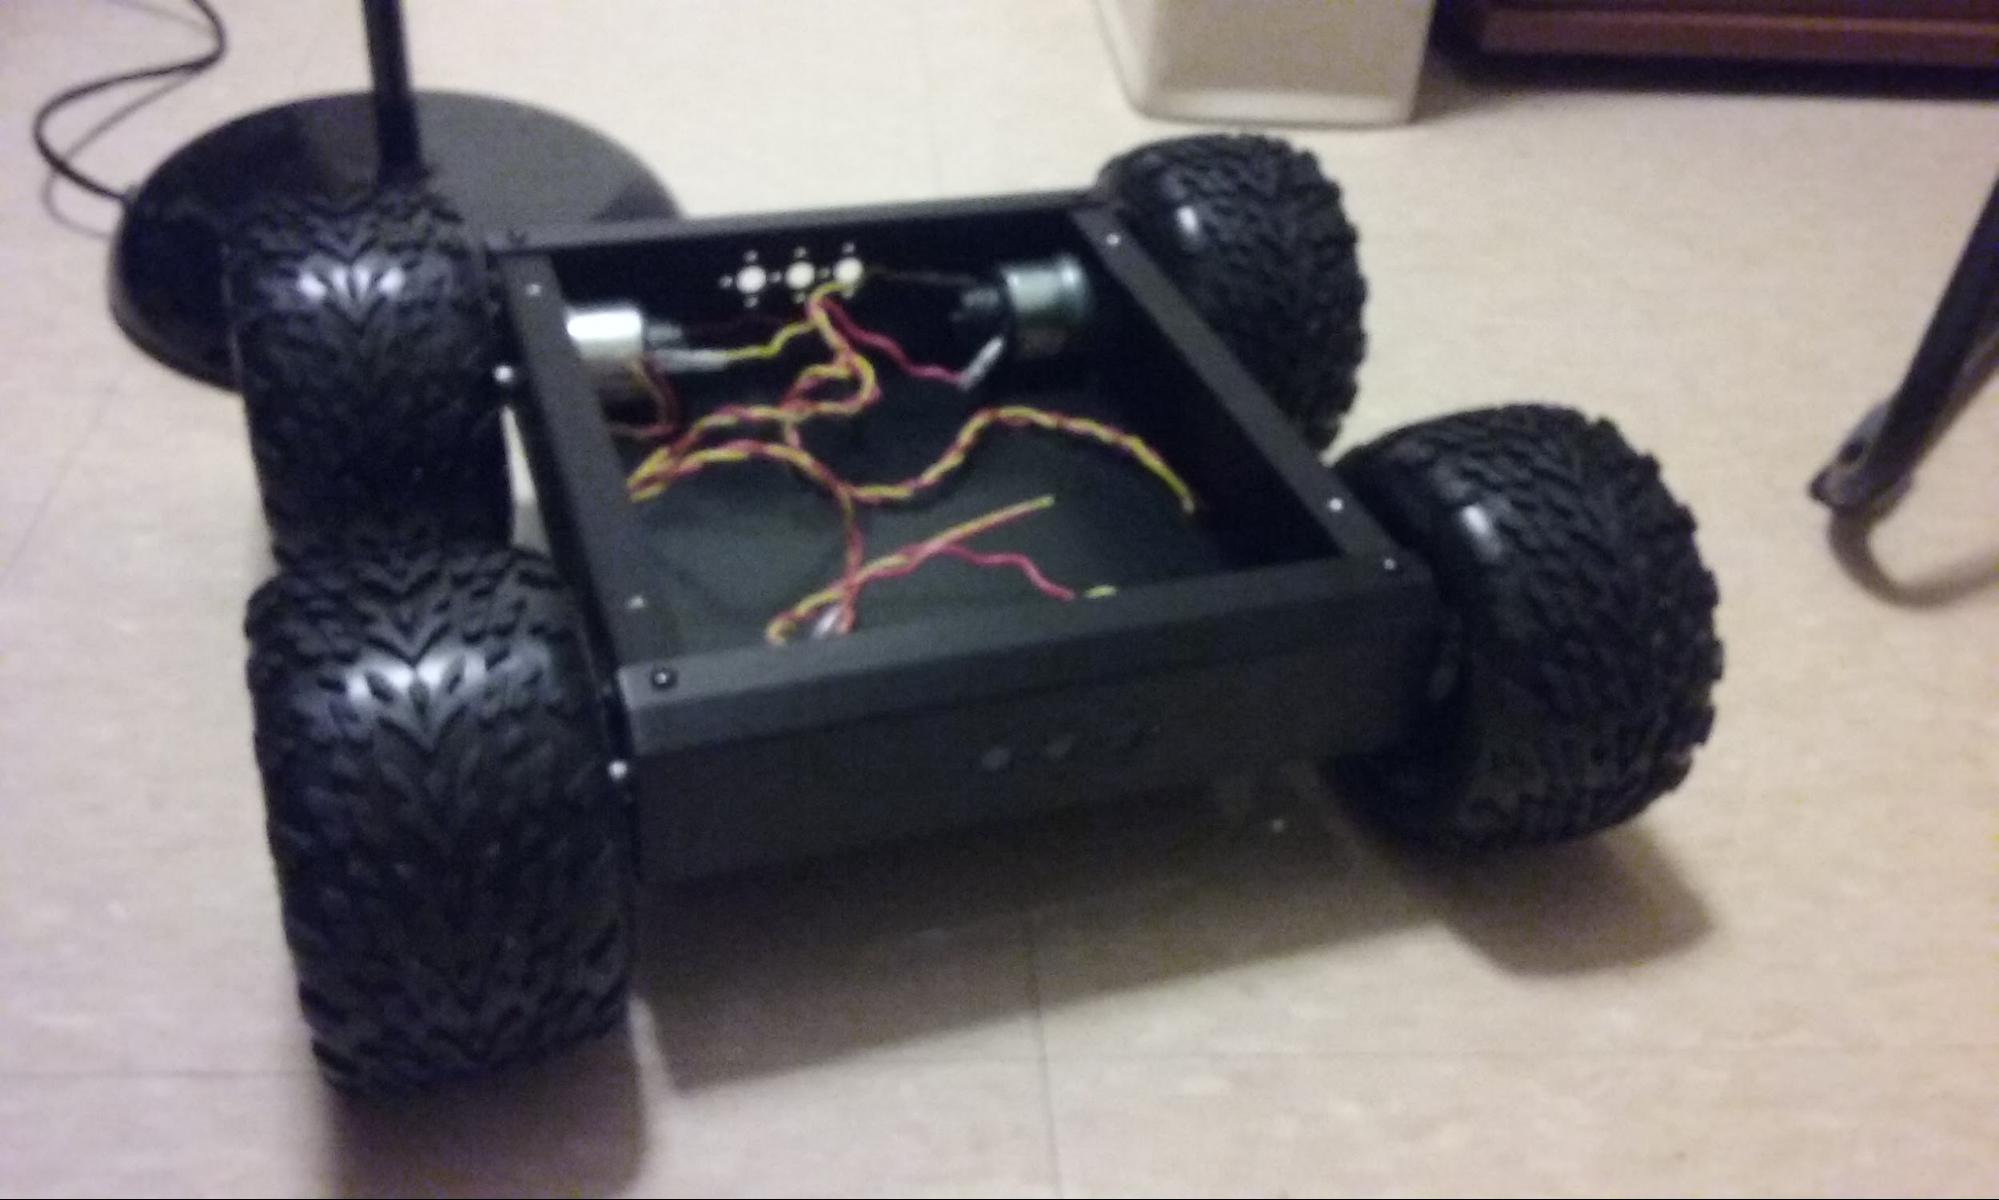
\includegraphics[width=0.5\textwidth]{chassis-constructed}
	\label{FigConstructedChassis}
\end{wrapfigure}

Figure \ref{FigConstructedChassis} shows the base just after assembly. The aluminum side brackets' mounting holes did not line up properly with the motors, so a Dremel drill was used to widen them.

\begin{wrapfigure}{R}{0.5\textwidth}
	\caption{Pieces Mounted}
	\centering
	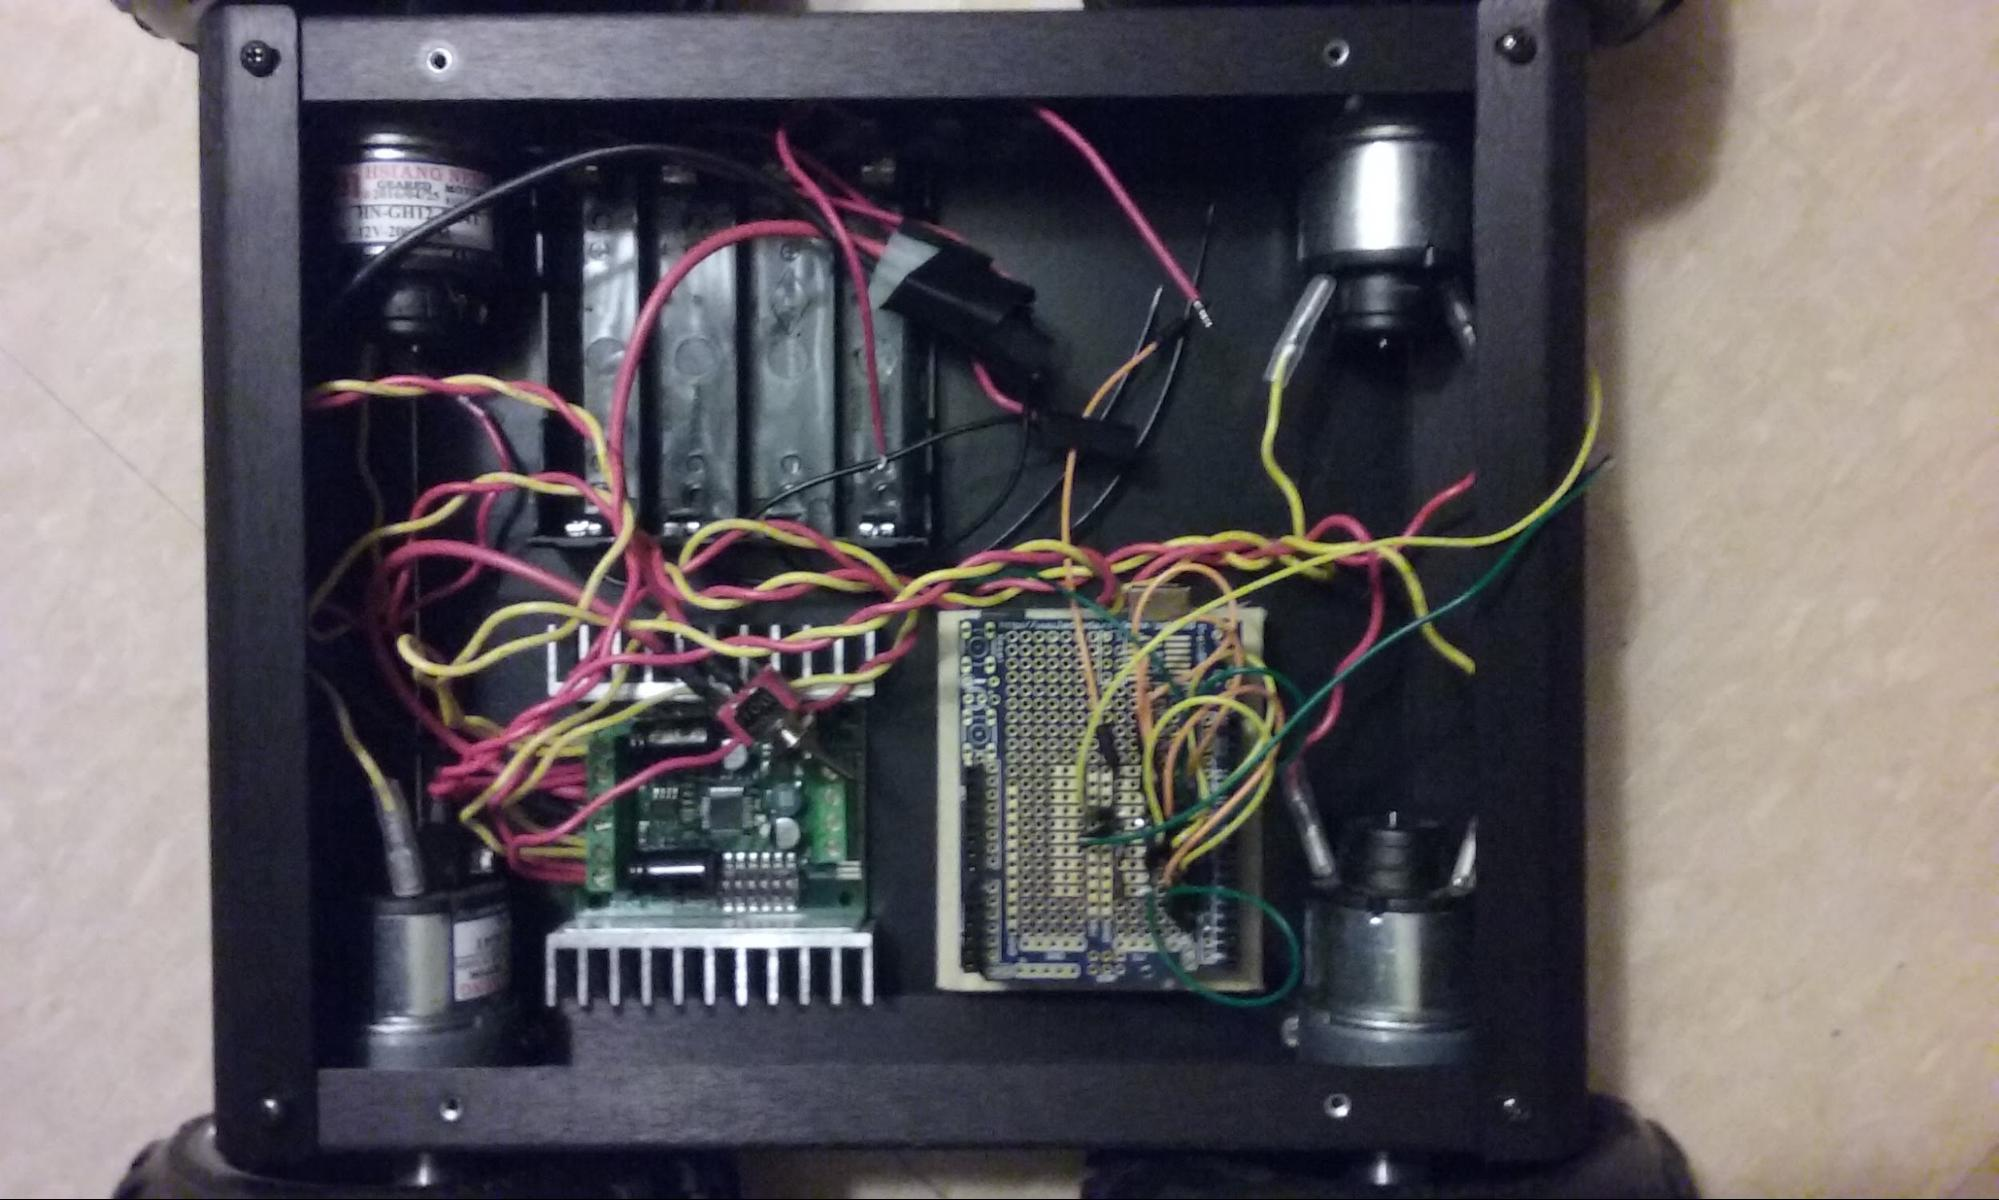
\includegraphics[width=0.5\textwidth]{chassis-parts-mounted}
	\label{FigChassisParts}
\end{wrapfigure}

The Arduino Uno was screwed to a 2.5" x 3" x 0.5" wooden poplar block, with non-conductive nylon washers placed between the screw head and the Uno, and between the Uno and the wooden block. The wooden Arduino mounting board and the motor driver were both attached via double-sided foam mounting tape to the bottom panel of the rover. The battery holder was attached with glue dots for easier removal.

\begin{wrapfigure}{L}{0.5\textwidth}
	\caption{Construction Finished}
	\centering
	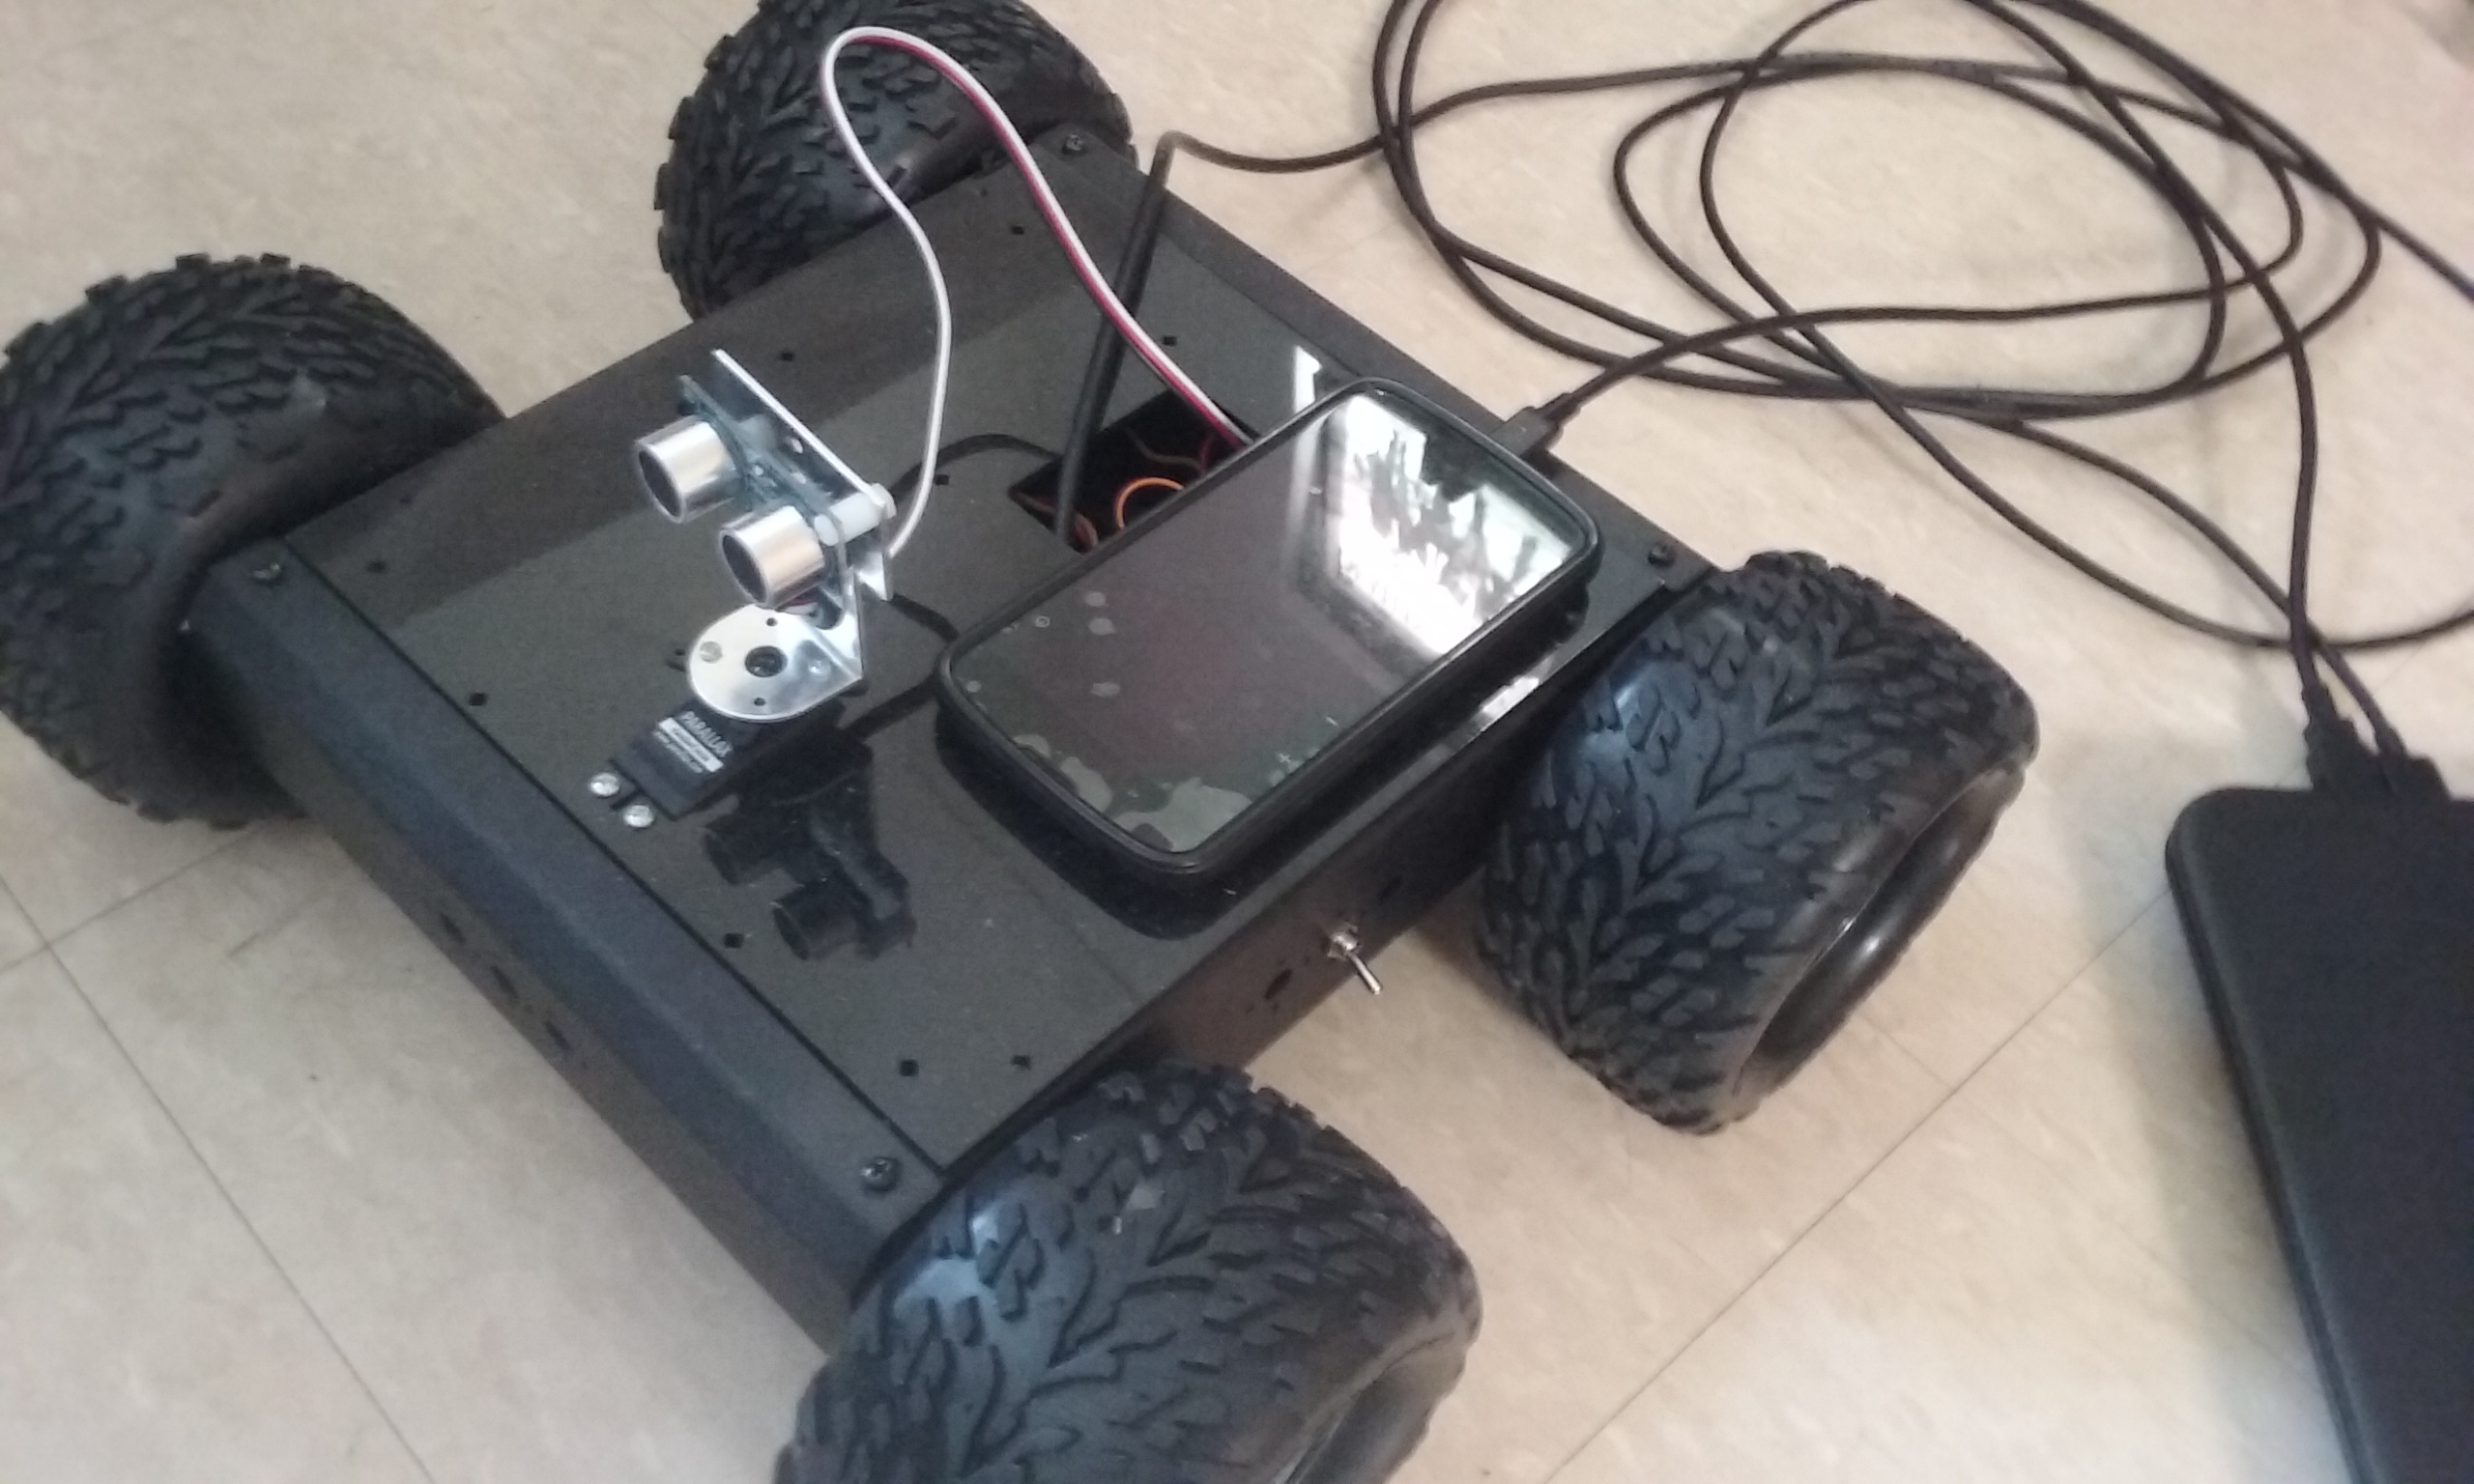
\includegraphics[width=0.5\textwidth]{roverFinished}
	\label{FigRoverFinished}
\end{wrapfigure}

The servo fits conveniently into a pre-cut opening in the top chassis panel, and is held in place with four 3mm x 6mm screws and corresponding washers. A mounting bracket is attached to the servo, and the PING))) sensor is screwed to that mounting bracket, using non-conductive washers and screws to separate the circuit board and the metal mounting bracket.

Another opening in the top panel allows the PING))) sensor to connect to the Arduino inside the body of the rover. This opening also allows the USB cable connected to the Arduino to reach the laptop. The smartphone sits on the top panel just to the left of this opening, secured in place by removable glue adhesive dots. It is also connected to the laptop via a micro-USB to USB cable.

\begin{figure}[p] 
	\caption{Electrical Connections}
	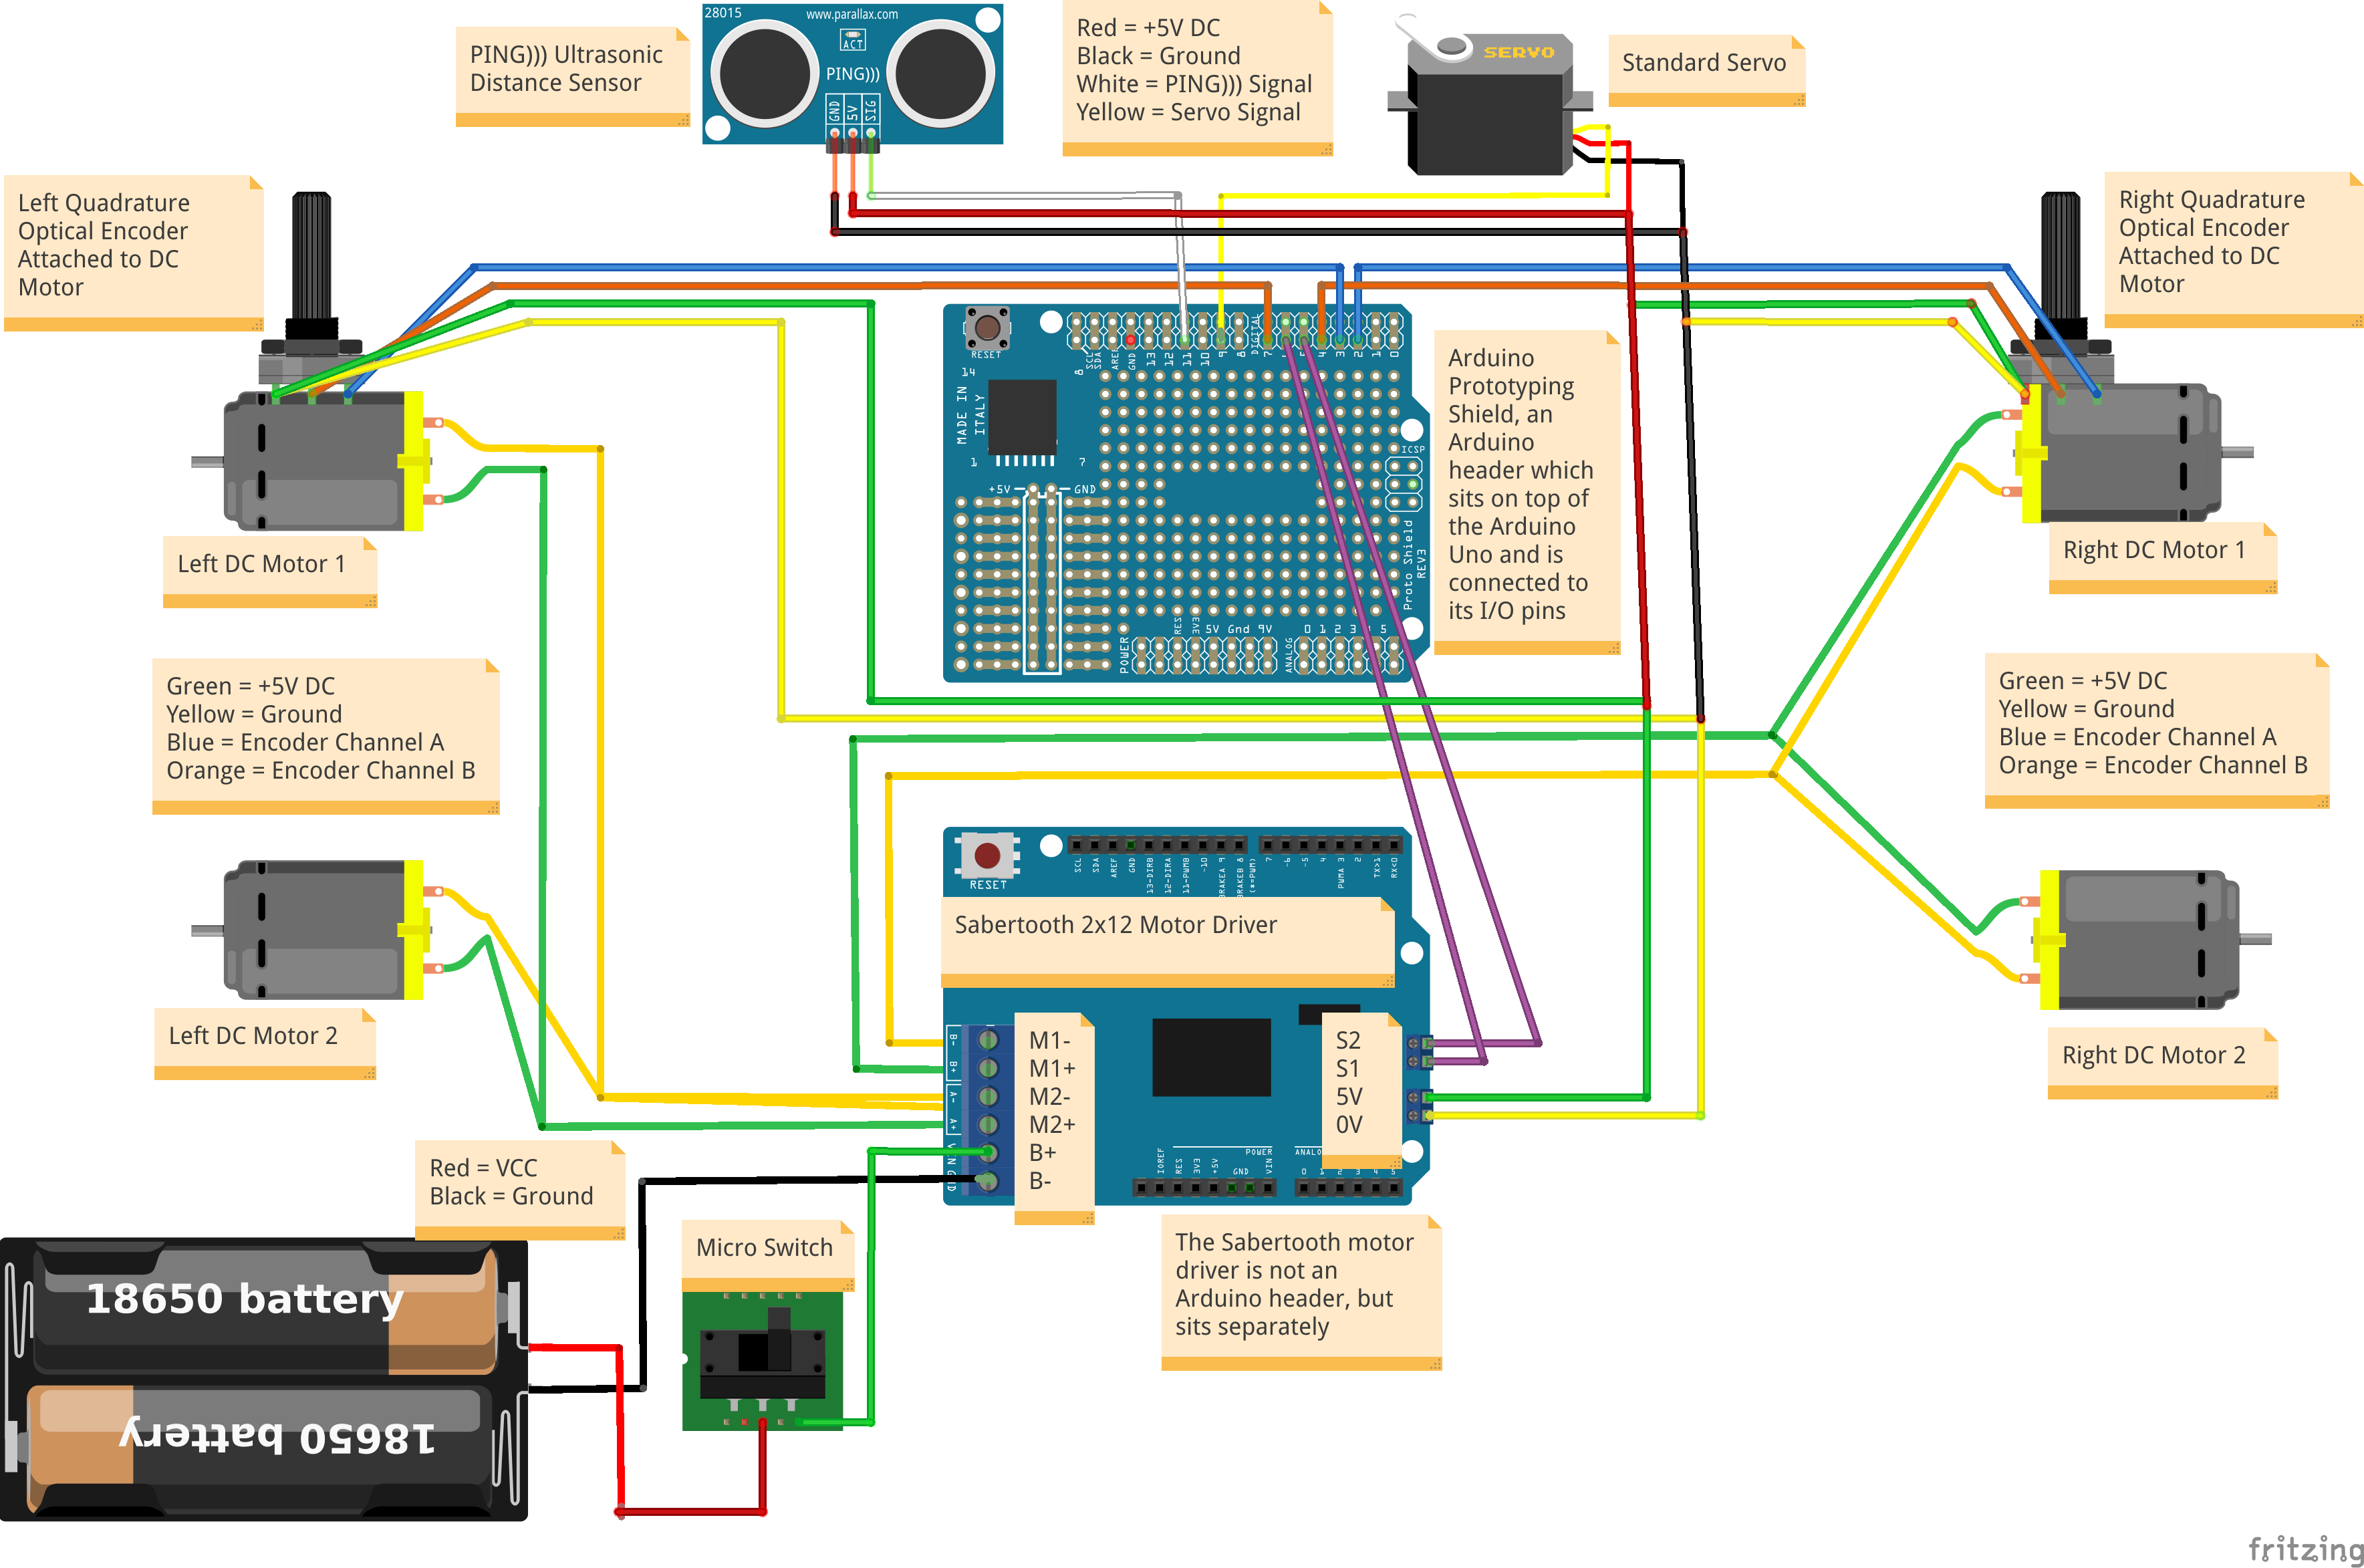
\includegraphics[width=\textwidth,height=\textheight,keepaspectratio, angle=90]{RoverDesign}
	\centering
	\label{figRoverDesign}
	\text{This image was created with Fritzing}
\end{figure}

For the configuration of electrical connections between parts, see Figure \ref{figRoverDesign}. These connections were made with flexible stranded core, 22 AWG breadboard wire. Connections to the Arduino's digital pins were made indirectly. A prototyping shield was stacked on top of the Arduino, and connected to its digital pins via pin headers. Signal pins were then soldered to the prototyping shield. Breadboard wires needing direct connection ideally should use terminal block connectors. However, these were difficult to find at a reasonable price, and so wires were soldered together tip to tip, and simply wrapped in electrical tape.

\section{Power}
Refer once more to Figure \ref{figRoverDesign} for a visual depiction of the power connections described here.

Besides the Arduino Uno, which is powered separately by a USB connection to the laptop, most of the rover's components are powered through the battery pack. This pack contains two individual 18650 lithium-ion cells connected in series. The battery pack is then connected to the motor driver's battery terminals B+ and B-. The positive B+ output goes through a microswitch, which is attached to one of the rover's side brackets, and is accessible from the outside. This acts as a kill switch for the battery pack.

The battery pack powers the motor driver, and excess power is then routed through the Sabertooth's on-board battery eliminator circuit (BEC). The BEC efficiently regulates the incoming voltage down to 5V, which is what the other electronics expect. The BEC outputs are labeled 0V and 5V in Figure \ref{figRoverDesign}. The ultrasonic sensor, its servo, and the two motor encoders are all powered through this BEC. The Arduino is also connected to this BEC's ground, as the microcontroller and motor driver must share a common ground plane in order for control signals to be correctly interpreted \cite{sabertoothUserGuide}. It is important to note that a BEC of some kind is essential in this project, as the Arduino's on-board 5V regulator can not handle the peak amperage draw of the servo.

Lithium ion cells hold 4.2V at full charge, and discharge down to a minimum of 2.7V. The Sabertooth has a lithium cutoff mode which senses the average voltage of cells in the battery pack, and shuts the driver down when that average dips below 3.0V. Cells connected in series add their voltage, so the voltage supplied through the motor driver's output channels will range from 8.4V to 6.0V, which is within the acceptable operating range for the DC motors. The specific li-ion cells being used can supply up to 20A continuously, and the motor driver can handle up to 12A per channel. The motors each draw a maximum current of 1.5A, and two are used per channel, putting the total possible current draw at 3A per channel, well below the limits of the motor driver and battery pack.

The BEC supplying power to the sensors is capable of supplying up to 1 Amp of continuous current, and 1.5 Amps of peak current. The ultrasonic sensor and the two motor encoders combined use less than 500 mA. However the standard servo - while normally drawing less than 500 mA itself -  has the potential to draw peak currents of up to 1A if it hits a snag and is stopped from moving. The sensors are therefore pushing the limits of the BEC's operating range. It is also important to check that the wires connected to the BEC are capable of handling the peak current without burning out. 22 AWG wires with 43 or more internal cores are rated to handle up to 1A of current. The rover's 22 AWG breadboard wires have a bit less than 43 internal cores, but have yet to have any issues. But the servo has not been under full load by being stopped, and so the wires have not truly been tested. Ideally those replicating this construction will use larger wires rated for higher current, to be safe.

Note that when using the rover, the sensors attached to the Arduino should be powered off first, else the Arduino may try to power itself via its input pins. The sensors are powered from the BEC on the motor driver, so they may be turned off by flipping the microswitch between the battery pack and motor driver.
